\documentclass[11pt]{article}
\usepackage[a4paper,margin=27mm]{geometry}
\usepackage[T1]{fontenc}
\usepackage{lmodern,microtype,amsmath,amssymb,amsthm,mathtools,enumitem,comment}
\usepackage{tikz}
\usepackage{xcolor}
\newcommand{\chg}[1]{{\color{red}#1}}
\usepackage{comment}
\usetikzlibrary{arrows.meta,calc}
\usepackage[most]{tcolorbox}
\usepackage[font=small,labelfont=bf]{caption}
\usepackage[colorlinks=true,linkcolor=blue,citecolor=blue,urlcolor=blue]{hyperref}



\colorlet{wone}{blue!70!black}
\colorlet{wtwo}{orange!85!black}
\colorlet{wthree}{green!50!black}
\colorlet{aone}{blue!22}
\colorlet{atwo}{orange!32}
\colorlet{athree}{green!22}

\newtcolorbox{stmt}[1]{enhanced,breakable,colback=white,colframe=black!55,boxrule=0.5pt,arc=1pt,
  left=5pt,right=5pt,top=3pt,bottom=3pt,fonttitle=\bfseries\small,coltitle=black,colbacktitle=black!8,title={#1}}
\DeclareRobustCommand{\stp}[1]{\tikz[baseline=(n.base)]\node[circle,draw,inner sep=0.7pt,minimum size=11pt,font=\scriptsize\bfseries](n){#1};}
\newenvironment{steps}{\begin{enumerate}[label=\stp{\arabic*},leftmargin=*,itemsep=2pt]}{\end{enumerate}}



\hypersetup{pdftitle={Coherence and Dominance under General Rankings}}

\newtheorem{theorem}{Theorem}[section]
\newtheorem{lemma}[theorem]{Lemma}
\newtheorem{proposition}[theorem]{Proposition}
\newtheorem{corollary}[theorem]{Corollary}
\theoremstyle{definition}
\newtheorem{definition}[theorem]{Definition}
\newtheorem{example}[theorem]{Example}
\theoremstyle{remark}
\newtheorem{remark}[theorem]{Remark}

\newcommand{\F}{\mathcal F}
\newcommand{\G}{\mathcal G}
\newcommand{\M}{\mathcal M}
\newcommand{\C}{\mathcal C}
\newcommand{\U}{\mathcal U}
\newcommand{\Lf}{\mathfrak L}
\newcommand{\supp}{\operatorname{supp}}
\newcommand{\cl}{\operatorname{cl}}
\setlist{itemsep=1pt,topsep=3pt}

\title{Dominance Generalised}
\author{Jason Konek}
\date{}

\begin{document}
\maketitle

\begin{abstract}
Here's a pretty little abstract. It's such a pretty little abstract. It does everything you want an abstract to do. It's a real eye-catcher. And it lets the reader know just what they're in for.

\end{abstract}




\section{Introduction}\label{sec:intro}


Dominance arguments are commonly used to justify the claim that some axioms or other are requirements of rationality. For example, De~Finetti argued that an agent's forecasts or estimates of bounded random variables ought to be probabilistic expectations \cite[\S1.6, \S3.3]{deFinetti1974}. This is necessary and sufficient for any finite collection of those estimates to avoid uniform dominance when evaluated using a loss function known as the Brier score. A finite set of estimates is uniformly dominated if there is some alternative set of forecasts/estimates that is guaranteed to get a smaller penalty (according to the loss function). Dominance seems to indicate a structural defect along whatever dimension of evaluation the loss function tracks. If the Brier score tracks a dimension of evaluation that is of cardinal importance to rationality, then forecasts/estimates that are dominated are plausibly rationally impermissible. Hence non-probabilistic estimates are rationally impermissible. Probabilistic estimates, in contrast, are rationally permissible (or at least they pass every test the dominance argument considers).


A number of authors have provided dominance arguments for coherence norms like probabilism~\cite{Joyce2009,Predd2009,SSK2009,Pettigrew2022,Nielsen2023}, norms governing updating like conditionalization~\cite{Briggs2020,Nielsen2021}, and deference norms like the Principal Principle~\cite[Chapter~10]{Pettigrew2016}. As elegant and insightful as these arguments are, they also muddle together some things that we really ought to keep distinct. De~Finetti's argument uses the Brier score. The arguments mentioned just above use a family of loss functions known as \textit{proper scoring rules}. They also assume a range of technical constraints, \textit{e.g.}, additivity, continuity, etc. (exactly which assumptions are in play vary from argument to argument). The various axioms on loss functions play two different roles. Firstly, they are meant to justify the claim that the loss function tracks a dimension of evaluation that is of cardinal importance to rationality. For example, most arguments listed here assume that loss function are \textit{truth-directed}, in the sense that moving an agent's estimates uniformly closer to the truth decreases the penalty that they receive. This seems non-negotiable if the loss function is to count as a measure of \textit{accuracy}. And facts about accuracy plausibly explain facts about epistemic rationality. Secondly, the ``core'' axioms (meant to capture the type of evaluation in play) together with the ``merely technical'' axioms jointly ensure that the loss functions in question have the structure needed for the dominance argument to work.

These two different roles should be kept separate. It is important to have a clear sense of whether there is some common structure that drives all (or most) extant variants of dominance arguments, and if so, what it is. That way, we can clearly distinguish which axioms on loss functions (i) only serve to pin down a relevant dimension of evaluation, (ii) which do this and also supply some requisite structure (and what structure they supply), and (iii) which are merely structural or technical axioms needed to make the dominance argument run. Indeed, we should really apply this thought to every modelling choice that goes into the dominance argument. The choice to use real-valued loss functions, for example, to penalise performance along a given dimension of evaluation imports a lot of structure (it makes comparisons complete/total, transitive, Archimedean, etc.). Sorting out which assumptions are playing which roles is necessary to fully understand what is going on in any given argument. It is also important for providing new dominance arguments in new settings. For example, to provide a dominance argument for coherence axioms on \textit{imprecise} probability models, we need to know what structure would be required to run such an argument. We then need to identify either loss functions or more general loss ``rankings'' that track an important dimension of evaluation and (perhaps supplemented with technical axioms) supply the requisite structure. If we take axioms (\textit{e.g.}, propriety) from one setting (\textit{e.g.}, probabilism) and assume that we must impose a similar axiom in another setting (\textit{e.g.}, coherence for lower previsions or sets of desirable gambles) without clearly delineating what role they were playing in the original argument, we might be mislead into thinking that the task is impossible.


To that end, we will present dominance arguments in what we take to be their most general form. We will not assume anything whatsoever about how to model an agent's state of opinion, what makes such a state coherent, or how to evaluate those states. The aim is to identify the minimal structure needed to run a dominance argument.



\section{Framework}\label{sec:framework}

Let $\Omega$ be a nonempty set of \emph{worlds}. Let $\M$ be a non-empty set of models. We will not assume anything about what sorts of models live in $\M$. $\M$ could be a set of precise credence functions, or Dempster-Shafer belief functions, or comparative belief relations, or lower previsions, or partial preference relations, or sets of desirable gambles, or choice/rejection functions, or probability filters, or whatever else you like. Indeed, there is no need to think of the elements of $\M$ as uncertainty models \textit{per se}, or even \textit{models} at all. $\M$ is just an unstructured set of options or things---perhaps ice cream cones, or holiday packages, etc. But our target application is uncertainty models. So we will continue to talk about $\M$ as a set of uncertainty models.




A \emph{ranking} $L=(\preceq_\omega)_{\omega\in\Omega}$ is a family of binary relations on $\M$, one for each $\omega\in\Omega$. These relations measure how well a model performs at a given task in a world. We say that $c\preceq_\omega m$ just in case $c$ performs at least as well as $m$ at $\omega$. For example, if $\M$ is a set of decision models which make recommendations about how to choose, then $c\preceq_\omega m$ might reflect the fact that $c$ does a better job guiding choice than $m$ at $\omega$. We will not assume anything about what sort of task is at issue, or what dimension(s) of evaluation these relations reflect. For general $\M$ (ice cream cones, holiday packages, etc.), the relations $\preceq_\omega$ just capture some way in which the options are better or worse at a world $\omega$.

The asymmetric part of a relation $\preceq_\omega$ is given by
\[
c\prec_\omega m\quad:\Longleftrightarrow\quad c\preceq_\omega m\ \text{and not}\ m\preceq_\omega c .
\]
Models $c$ and $m$ are \emph{equivalent} if $c\preceq_\omega m$ and $m\preceq_\omega c$ for every $\omega$. At the outset, we do not assume anything about these relations (completeness, transitivity, reflexivity, etc.).

For any ranking $L$ and any models $c,m\in\M$, we say that $c$ \emph{dominates} $m$ if
\[
(\forall\omega\in\Omega)\ c\preceq_\omega m\qquad\text{and}\qquad(\exists\omega\in\Omega)\ m\not\preceq_\omega c .
\]
We say that $m$ is \emph{undominated under $L$} if no $c\in\M$ dominates it. $\U_L$ is the set of models in $\M$ undominated under $L$.

Let $\Lf$ be a putatively complete class of reasonable rankings. It contains all and only the reasonable rankings of models in $\M$. (To reiterate, we assume nothing substantive about what makes a ranking reasonable.) A model $m\in\M$ is
\begin{align*}
&\text{\emph{rationally permissible} (relative to $\Lf$)}&&\text{if }(\exists L\in\Lf)\ m\in\U_L;\\
&\text{\emph{irrational} (relative to $\Lf$)}&&\text{if }(\forall L\in\Lf)\ m\notin\U_L.
\end{align*}
That is, a model is rationally permissible if there is \textit{some} reasonable way of measuring performance which makes it come out undominated. It is irrational if \textit{every} reasonable way of measuring performance makes it come out dominated.

Here 
In what follows, we will make a few assumptions about the class $\Lf$ of reasonable rankings.

\chg{Firstly}, we assume that there is some class $\C\subseteq\M$ of ``coherent'' models that are ``not obviously suboptimal'' at the relevant task. We do not assume anything substantive about coherence. It is just a special status that a model can have. Any model that is not coherent is \emph{incoherent}. 


\chg{Secondly}, for each reasonable ranking $L\in\mathfrak L$, we assume that there is a nonempty, maximal class of coherent models, $\C_L\subseteq\chg{\C}$, which $L$ deems ``not obviously suboptimal'' in the sense of being \textit{undominated}.
\begin{enumerate}[label=\textbf{(LA)},leftmargin=*]
\item \textbf{Ranking-specific admissibility.} $\C_L\coloneqq \C\cap\U_L\neq\varnothing$.
\end{enumerate}

\chg{Thirdly}, the rankings $L\in\mathfrak L$ collectively render \textit{all} coherent models undominated.
\begin{enumerate}[label=\textbf{(CA)},leftmargin=*]
\item \textbf{Coherent admissibility.} $\C=\bigcup_{L\in\mathfrak L}\C_L$.
\end{enumerate}

Now choose a reasonable ranking $L\in\mathfrak L$. By definition $\C_L\subseteq\U_L$. That is, the coherent undominated models (relative to $L$) are undominated. Given coherent admissibility (CA), this entails that every coherent model is rationally permissible. But (LA) does \textit{not} rule out the possibility that additional, incoherent models are undominated as well, and hence also rationally permissible. That is, we do not simply \textit{assume} that incoherent models are defective, in the sense of being dominated relative to all reasonable rankings. The job of the dominance argument below is to \textit{prove} this stronger claim given one additional assumption.







\section{Important lemmas}\label{sec:lemmas}

\subsection{Finitely additive probability}\label{sec:prob}

For any finite nonempty set of worlds $F\subseteq\Omega$, let $\Delta_F\coloneqq\{p\in[0,1]^F:\sum_{\omega\in F}p_\omega=1\}$ be the set of probability mass functions on $F$ equipped with the Euclidean topology. Let $p_\omega\coloneqq p(\{\omega\})$. Let $\supp p\coloneqq\{\omega\in F:p_\omega>0\}$ be the \textit{support of p}, \textit{i.e.}, the set of worlds in $F$ that have positive probability relative to $p$. Let $\delta_\omega\in\Delta_F$ be the indicator function which gives probability $1$ to $\omega$ and $0$ to every other world.

Let $\Delta$ be the set of \emph{finitely additive probabilities} on the power set of $\Omega$, $2^\Omega$. 

\begin{definition}\label{def:finitely-additive-probability}
A map $p:2^\Omega\to[0,1]$ is a \emph{finitely additive probability function} iff:
\begin{enumerate}[label=\textup{(FA\arabic*)}]
  \item $p(\Omega)=1$;
  \item $p(E)\geq p(\varnothing)$;
  \item if $E\cap F=\varnothing$, then $p(E\cup F)=p(E)+p(F)$.
\end{enumerate}
\end{definition}

$\Delta$ comes equipped with the product topology. Just as with probability mass functions, let $p_\omega\coloneqq p(\{\omega\})$ and $\supp p\coloneqq\{\omega:p_\omega>0\}$.  $p$ is \emph{finitely supported} if $p(F)=1$ for some finite $F\subseteq\Omega$. Finitely additive probabilities need not be countably additive, need not be finitely supported, and indeed need not give positive probability to any world. For any finite $F\subseteq\Omega$ and probability mass function $p\in\Delta_F$, we can use $p$ to generate a unique finitely additive probability $2^\Omega$ in the obvious way, \textit{viz.}, $p(A):=\sum_{\omega\in A\cap F}p_\omega$.


Walley (1991: Theorems~3.2.2--3.2.3) shows that any finitely additive probability generates a unique \textit{finitely additive expectation} and vice versa. Let $\G$ be the set of all ``gambles'' or bounded random variables $g:\Omega\to\mathbb R$.


\begin{definition}\label{def:finitely-additive-expectation}
A map $P\colon\G\to\mathbb R$ is a \textit{finitely additive expectation} or \textit{linear prevision} iff:
\begin{enumerate}[label=\textup{(LNP\arabic*)}]
  \item $P(\mathbf{1}_\Omega)=1$;
  \item if $f\leq g$ (\textit{i.e.}, $f(\omega)\leq g(\omega)$ for all $\omega\in\Omega$) then $P(f)\leq P(g)$;
  \item $P(cf)=c\,P(f)$ for all $c>0$;
  \item $P(f+g)=P(f)+P(g)$.
\end{enumerate}
\end{definition}

A \emph{simple gamble} is a gamble of the form $f=\sum_{i=1}^{n}\alpha_i\,\mathbf{1}_{E_i}$ where $E_1,\ldots,E_n$ partition $\Omega$. For a finitely additive probability $p$, the expectation of a simple gamble is defined as:
\[
  E_p(f) \;:=\; \sum_{i=1}^{n}\alpha_i\,p(E_i).
\]
This suffices to fix the value of the unique linear prevision $E_p$ generated by $p$ for \textit{any} gamble. In general, $E_p(f)=\lim_jE_p(f_j)$ for any sequence of simple gambles $f_j\to f$.


There are a few well-known facts about finitely additive probabilities that we will need later and state here without proof.


\begin{lemma}\label{lem:prob}
\leavevmode
\begin{enumerate}[label=(\alph*)]
\item $\Delta$ is compact.
\item For every finite nonempty $F\subseteq\Omega$, let $\iota_F:\Delta_F\to\Delta$ defined by $\iota_F(p)(A):=\sum_{\omega\in A\cap F}p_\omega$. Then $\iota_F$ is continuous, injective and preserves supports, \textit{i.e.}, $\supp p = \supp \iota_F(p)$. Its image is $\{p\in\Delta:p(F)=1\}$. If $\Omega$ is finite, $\iota_\Omega$ is a homeomorphism onto $\Delta$.
\item For any $g\in\G$, the map $p\mapsto E_p(g)$ is continuous. 
\end{enumerate}
\end{lemma}



\subsection{KKM lemma}\label{sec:kkm}

The theorem that drives the general dominance argument is a seminal result of Knaster--Kuratowski--Mazurkiewicz {\cite{KKM1929}}.

\begin{lemma}\label{lem:kkm}
Let $F$ be finite and nonempty, and let $(A_\omega)_{\omega\in F}$ be closed subsets of $\Delta_F$ such that every $p\in\Delta_F$ lies in $A_\omega$ for some $\omega\in\supp p$. Then $\bigcap_{\omega\in F}A_\omega\ne\varnothing$.
\end{lemma}


\begin{comment}
\begin{proof}
The hypothesis at $\delta_\omega$ gives $\delta_\omega\in A_\omega$, so each $A_\omega$ is nonempty and compact. Define
\[
d_\omega(p)\coloneqq\min_{q\in A_\omega}\|p-q\|,\qquad s(p)\coloneqq\sum_{\omega\in F}d_\omega(p),\qquad \Psi(p)_\omega\coloneqq\frac{p_\omega+d_\omega(p)}{1+s(p)}.
\]
$\Psi:\Delta_F\to\Delta_F$ is continuous. At a Brouwer fixed point $p$, $p_\omega s(p)=d_\omega(p)$ for every $\omega$. Choose $\omega$ with $p_\omega>0$ and $p\in A_\omega$. Then $d_\omega(p)=0$, so $s(p)=0$, so every $d_\omega(p)=0$ and $p\in\bigcap_{\omega\in F}A_\omega$.
\end{proof}
\end{comment}






\begin{figure}[ht]
\centering
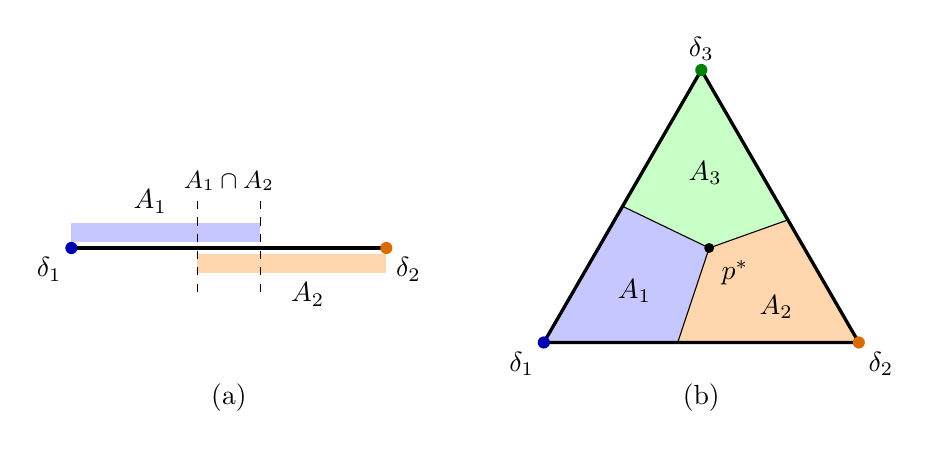
\begin{tikzpicture}
\begin{scope}[yshift=1.2cm]
 \fill[aone] (0,0.08) rectangle (2.4,0.32);
 \fill[atwo] (1.6,-0.32) rectangle (4,-0.08);
 \draw[very thick] (0,0) -- (4,0);
 \fill[wone] (0,0) circle (2.2pt); \fill[wtwo] (4,0) circle (2.2pt);
 \node[below left] at (0,0) {$\delta_1$};
 \node[below right] at (4,0) {$\delta_2$};
 \node[above] at (1.0,0.32) {$A_1$};
 \node[below] at (3.0,-0.32) {$A_2$};
 \draw[dashed] (1.6,0.6) -- (1.6,-0.6);
 \draw[dashed] (2.4,0.6) -- (2.4,-0.6);
 \node[above] at (2,0.6) {\small $A_1\cap A_2$};
 \node at (2,-1.9) {(a)};
\end{scope}
\begin{scope}[xshift=6cm]
 \coordinate (d1) at (0,0); \coordinate (d2) at (4,0); \coordinate (d3) at (2,3.46);
 \coordinate (e12) at (1.7,0); \coordinate (e23) at (3.1,1.557); \coordinate (e13) at (1,1.73);
 \coordinate (c) at (2.1,1.2);
 \fill[aone] (d1)--(e12)--(c)--(e13)--cycle;
 \fill[atwo] (d2)--(e23)--(c)--(e12)--cycle;
 \fill[athree] (d3)--(e13)--(c)--(e23)--cycle;
 \draw[very thick] (d1)--(d2)--(d3)--cycle;
 \draw (e12)--(c) (e23)--(c) (e13)--(c);
 \fill[wone] (d1) circle (2.2pt); \fill[wtwo] (d2) circle (2.2pt); \fill[wthree] (d3) circle (2.2pt);
 \node[below left] at (d1) {$\delta_1$};
 \node[below right] at (d2) {$\delta_2$};
 \node[above] at (d3) {$\delta_3$};
 \node at (1.15,0.65) {$A_1$};
 \node at (2.95,0.45) {$A_2$};
 \node at (2.05,2.15) {$A_3$};
 \fill (c) circle (1.8pt) node[below right=1pt] {$p^*$};
 \node at (2,-0.7) {(b)};
\end{scope}
\end{tikzpicture}
\caption{The hypothesis of Lemma~\ref{lem:kkm}: $\delta_\omega\in A_\omega$; each face is covered by the sets indexed by its vertices. (a) $|F|=2$. (b) $|F|=3$.}
\label{fig:kkm}
\end{figure}






\section{The selection theorem}\label{sec:selection}

\begin{definition}[Selection data]\label{def:selection-data}
Let $L$ be a ranking and $x\in\chg{\M}$. \emph{Selection data for $x$} consist of a map $c:\Delta\to\chg{\M}$, whose values $c(p)$ are the \emph{candidates}, and closed sets $A_\omega\subseteq\Delta$, $\omega\in\Omega$, such that:
\begin{enumerate}[label=(S\arabic*),leftmargin=3em]
\item\label{S1} for every $\omega\in\Omega$ and every $p\in A_\omega$: $c(p)\preceq_\omega x$;
\item\label{S2} for every finitely supported $p\in\Delta$ there is $\omega\in\Omega$ with $p_\omega>0$ and $p\in A_\omega$;
\item\label{S3} for every $p\in\bigcap_{\omega\in\Omega}A_\omega$ there is $\omega\in\Omega$ with $x\not\preceq_\omega c(p)$.
\end{enumerate}
\end{definition}

\begin{theorem}[Selection theorem]\label{thm:selection}
Let $\Omega$ be any nonempty set, $L$ any ranking and $x\in\chg{\M}$. If selection data for $x$ exist, then $\bigcap_\omega A_\omega\ne\varnothing$, and $c(p)$ dominates $x$ for every $p\in\bigcap_\omega A_\omega$.
\end{theorem}
\begin{proof}
Let $G\subseteq\Omega$ be finite and nonempty, and $\iota_G$ as in Lemma~\ref{lem:prob}(b). The sets $\iota_G^{-1}(A_\omega)$, $\omega\in G$, are closed in $\Delta_G$. Let $\lambda\in\Delta_G$. Then $\iota_G(\lambda)$ is finitely supported, so by \ref{S2} some $\omega$ has $\iota_G(\lambda)_\omega>0$ and $\iota_G(\lambda)\in A_\omega$. Since $\iota_G$ preserves supports, $\omega\in\supp\lambda\subseteq G$ and $\lambda\in\iota_G^{-1}(A_\omega)$. By Lemma~\ref{lem:kkm}, $\bigcap_{\omega\in G}\iota_G^{-1}(A_\omega)$ contains a point $\lambda^*$, and $\iota_G(\lambda^*)\in\bigcap_{\omega\in G}A_\omega$. So the closed sets $A_\omega$ have the finite intersection property. If $\bigcap_\omega A_\omega$ were empty, the open sets $\Delta\setminus A_\omega$ would cover the compact space $\Delta$ (Lemma~\ref{lem:prob}(a)); finitely many would cover it, and the corresponding finite intersection would be empty. Hence there is $p\in\bigcap_\omega A_\omega$. By \ref{S1}, $c(p)\preceq_\omega x$ for every $\omega$, and by \ref{S3} there is $\omega$ with $x\not\preceq_\omega c(p)$.
\end{proof}

The candidates in Definition~\ref{def:selection-data} are arbitrary, so the dominator that Theorem~\ref{thm:selection} produces may itself be dominated. When the candidates are known to be undominated, the theorem gives more.

\begin{corollary}[Undominated dominators]\label{cor:undominated-dominators}
Let $c$ and $(A_\omega)_{\omega\in\Omega}$ be selection data for $x$, and suppose $c(p)\in\U_L$ for every $p\in\bigcap_{\omega\in\Omega}A_\omega$. Then $x$ has an undominated dominator: $c(p)$ for any $p\in\bigcap_\omega A_\omega$. If moreover $c(p)\in\C$ for every such $p$, then $x$ is dominated by a member of $\C\cap\U_L$. Both hypotheses hold if $c(p)\in\C\cap\U_L$ for every $p\in\Delta$.
\end{corollary}
\begin{proof}
By Theorem~\ref{thm:selection}, $\bigcap_\omega A_\omega\neq\varnothing$ and $c(p)$ dominates $x$ for every $p$ in it. By hypothesis $c(p)\in\U_L$, and in the second case $c(p)\in\C\cap\U_L$.
\end{proof}

\begin{lemma}[Sufficient conditions for (S3)]\label{lem:S3}
Let $c$ and closed sets $A_\omega$ satisfy \ref{S1}. Then \ref{S3} holds if either
\begin{enumerate}[label=(\alph*)]
\item no candidate $c(p)$ is tied with $x$ at every world; or
\item $x\not\preceq_\omega c(p)$ whenever $p\in A_\omega$.
\end{enumerate}
\end{lemma}
\begin{proof}
Let $p\in\bigcap_\omega A_\omega$; by \ref{S1}, $c(p)\preceq_\omega x$ for every $\omega$. (a) If also $x\preceq_\omega c(p)$ for every $\omega$, the two would be tied at every world. (b) Take any $\omega$.
\end{proof}

\begin{definition}[Fixed and countable selection]
For $I\subseteq\chg{\M}$, \emph{fixed selection} means that there exists a map $c:\Delta\to\chg{\M}$ such that every $x\in I$ has selection data with candidate map $c$. \emph{Countable selection} means that there exists a sequence $(c^j)_{j\in\mathbb N}$ of such maps such that every $x\in I$ has selection data with candidate map $c^j$ for some $j$.
\end{definition}

\begin{theorem}[Complete-class theorem]\label{thm:complete-class}
Let $\Lf$ be a \chg{nonempty} family of rankings and consider:
\begin{enumerate}
\item[(X)] \emph{Exclusion}: for every $L\in\Lf$ and every incoherent $x\in\chg{\M}$, selection data for $x$ exist;
\item[(A)] \emph{Coherent coverage}: for every $c\in\C$ there is $L\in\Lf$ with $c\in\U_L$\chg{.}
\end{enumerate}
\begin{enumerate}[label=(\alph*)]
\item Under (X), every incoherent model is dominated under every ranking in $\Lf$; so every incoherent model is irrational, and $\U_L=\C_L$ for every $L\in\Lf$.
\item Under (X) and (A), the rationally permissible models are exactly the coherent models, and the irrational models are exactly the incoherent models.
\end{enumerate}
\end{theorem}
\begin{proof}
(a) Let $L\in\Lf$ and $x\in\chg{\M}$ incoherent. By (X) and Theorem~\ref{thm:selection}, $x$ is dominated under $L$, so $x\notin\U_L$; as $L$ was arbitrary, $x$ is irrational. Hence $\U_L\subseteq\C\cap\U_L=\C_L\subseteq\U_L$.
(b) By (a) no incoherent model is permissible; by (A) every coherent model is. Permissible and irrational are complementary.
\end{proof}

\section{Applications to accuracy}\label{sec:applications}

In this section a ranking is given by a \emph{loss} $\ell:\chg{\M}\times\Omega\to[0,\infty]$, with $m\preceq_\omega m'$ iff $\ell(m,\omega)\le\ell(m',\omega)$. A function $f$ from a topological space to $[0,\infty]$ is \emph{lower semicontinuous} if $\{z:f(z)\le a\}$ is closed for every real $a$. For finite $\Omega$ write $E_p\ell(m,\cdot)\coloneqq\sum_\omega p_\omega\ell(m,\omega)$ with $0\cdot\infty=0$.

\begin{lemma}[Selection data for losses]\label{lem:loss-one-stage}
Let $L$ be given by a loss $\ell$, and let $p\mapsto c_p$ be a map $\Delta\to\chg{\M}$ such that:
\begin{enumerate}[label=(\roman*)]
\item for every $\omega$, $p\mapsto\ell(c_p,\omega)$ is lower semicontinuous on $\Delta$;
\item for every $m\in\chg{\M}$ and every finitely supported $p$, some $\omega$ with $p_\omega>0$ has $\ell(c_p,\omega)\le\ell(m,\omega)$.
\end{enumerate}
Let $x\in\chg{\M}$, $c(p)\coloneqq c_p$ and $A_\omega\coloneqq\{p\in\Delta:\ell(c_p,\omega)\le\ell(x,\omega)\}$. Then \ref{S1} and \ref{S2} hold. If no $c_p$ is tied at every world with $x$, then \ref{S3} holds, and some $c_p$ dominates $x$.
\end{lemma}
\begin{proof}
$A_\omega$ is closed by (i), and equals $\Delta$ if $\ell(x,\omega)=\infty$. \ref{S1} is the definition of $A_\omega$, and \ref{S2} is (ii) with $m=x$. \ref{S3} follows from Lemma~\ref{lem:S3}(a). Apply Theorem~\ref{thm:selection}.
\end{proof}

In each application below, the complete-class conclusion is Theorem~\ref{thm:complete-class} for the one-ranking family $\Lf=\{L\}$: (X) follows from Lemma~\ref{lem:loss-one-stage} and (A) from the stated protection argument.

The protection argument covers every candidate. In Propositions~\ref{prop:proper}, \ref{prop:probabilism}, \ref{prop:updating} and~\ref{prop:chance}, each candidate $c_p$ is coherent and is proved to be undominated. In Proposition~\ref{prop:updating} this is proved directly for every coherent strategy; it is not derived from Bayes optimality under the probability $q$ used for coverage. So $c_p\in\C\cap\U_L$ for every $p\in\Delta$. By Corollary~\ref{cor:undominated-dominators}, in each application every incoherent model is dominated by a coherent model that is itself undominated, namely $c_p$ for any $p\in\bigcap_\omega A_\omega$.

\subsection{Proper losses on finitely many worlds}

\begin{proposition}[{\cite{Predd2009,Pettigrew2022}}]\label{prop:proper}
Let $\Omega$ be finite, let $\ell$ be a loss on $\chg{\M}$, and let $p\mapsto c_p$ map $\Delta$ onto $\C\subseteq\chg{\M}$. Suppose each $c_p$ is the unique Bayes model for $p$, that is, $E_p\ell(c_p,\cdot)<E_p\ell(m,\cdot)$ for every $m\ne c_p$, and $p\mapsto\ell(c_p,\omega)$ is lower semicontinuous for every $\omega$. Then every incoherent model is dominated by some $c_p$, every coherent model is undominated, and $\{L\}$ satisfies \chg{(X) and (A)}.
\end{proposition}
\begin{proof}
If $\chg{\M}$ is a singleton $\{c\}$, then $c$ is coherent and there is nothing to prove. Otherwise $E_p\ell(c_p,\cdot)<\infty$ for every $p$, since $E_p\ell(c_p,\cdot)<E_p\ell(m,\cdot)$ for some $m$.

\emph{Weak dominators of $c_p$.} If $m\preceq_\omega c_p$ for every $\omega$, then $E_p\ell(m,\cdot)\le E_p\ell(c_p,\cdot)$, so $m=c_p$ by uniqueness. Hence no model dominates $c_p$, which gives (A) since the map is onto $\C$. Hence also no $c_p$ is tied at every world with an incoherent model, since such a model would weakly dominate $c_p$.

\emph{Coverage.} Let $m\in\chg{\M}$ and $p\in\Delta$ (every $p$ is finitely supported, by Lemma~\ref{lem:prob}(b)). If $\ell(c_p,\omega)>\ell(m,\omega)$ for every $\omega\in\supp p$, then, as $E_p\ell(c_p,\cdot)$ is finite, $E_p\ell(m,\cdot)<E_p\ell(c_p,\cdot)$, contradicting Bayes optimality. This is Lemma~\ref{lem:loss-one-stage}(ii), and (i) is assumed. For incoherent $x$, Lemma~\ref{lem:loss-one-stage} gives selection data; this is (X).
\end{proof}

\subsection{Probabilism on arbitrary domains}

Let $\Omega$ be arbitrary, $\chg{\M}=[0,1]^{2^\Omega}$ with the product topology, and $\C\coloneqq\Delta$, with the topology inherited from $\chg{\M}$. For $q\in\Delta$ and $f:\Omega\to[0,\infty]$ put $E_qf\coloneqq\sup_{k\in\mathbb N}E_q(f\wedge k)$. Applying Lemma~\ref{lem:prob}(c) to $f\wedge k$ and taking increasing limits gives, with $0\cdot\infty=0$,
\begin{gather*}
E_{ap+(1-a)q}f=aE_pf+(1-a)E_qf\quad(0<a<1),\\
p(F)=1,\ F\text{ finite}\ \Longrightarrow\ E_pf=\textstyle\sum_{\omega\in F}p_\omega f(\omega),
\end{gather*}
and $f\le f'$ implies $E_qf\le E_qf'$. The loss $\ell$ is \emph{quasi-strictly proper} if $E_q\ell(q,\cdot)\le E_q\ell(m,\cdot)$ for all $q\in\C$ and $m\in\chg{\M}$, strictly whenever $m\notin\C$.

\begin{proposition}[{\cite{Nielsen2023}}]\label{prop:probabilism}
If $\ell$ is quasi-strictly proper and each $q\mapsto\ell(q,\omega)$ is lower semicontinuous on $\Delta$, then every incoherent model is dominated by a member of $\Delta$, every member of $\Delta$ is undominated, and $\{L\}$ satisfies \chg{(X) and (A)}.
\end{proposition}
\begin{proof}
\emph{Finiteness.} For $q\in\C$, $E_q\ell(q,\cdot)<E_q\ell(m_0,\cdot)\le\infty$ for the incoherent $m_0\equiv0$, so $E_q\ell(q,\cdot)<\infty$.

\emph{(A).} Suppose $m$ dominates $q\in\C$, with $\ell(m,w)<\ell(q,w)$; in particular $\ell(m,w)<\infty$. Weak dominance and monotonicity give $E_q\ell(m,\cdot)\le E_q\ell(q,\cdot)$, and propriety gives equality, so $E_q\ell(m,\cdot)=E_q\ell(q,\cdot)<\infty$. For $k\ge2$ put $q_k\coloneqq(1-1/k)q+\delta_w/k\in\C$. Propriety at $q_k$ and at $q$ gives
\[
\tfrac1k\ell(q_k,w)+(1-\tfrac1k)E_q\ell(q,\cdot)\le E_{q_k}\ell(q_k,\cdot)\le E_{q_k}\ell(m,\cdot)=\tfrac1k\ell(m,w)+(1-\tfrac1k)E_q\ell(q,\cdot).
\]
Subtracting the finite common term gives $\ell(q_k,w)\le\ell(m,w)$ for every $k$. Since $q_k\to q$ in $\Delta$, lower semicontinuity gives $\ell(q,w)\le\ell(m,w)$, a contradiction.

\emph{Ties.} If an incoherent $m$ were tied at every world with $q\in\C$, then $E_q\ell(m,\cdot)=E_q\ell(q,\cdot)$, contradicting strict propriety against incoherent models.

\emph{Coverage.} Put $c_p\coloneqq p$ for $p\in\Delta$; Lemma~\ref{lem:loss-one-stage}(i) is the hypothesis. Let $p(F)=1$ for a finite $F$ and $m\in\chg{\M}$. Then $E_p\ell(p,\cdot)=\sum_{\omega\in F}p_\omega\ell(p,\omega)<\infty$, so $\ell(p,\omega)<\infty$ for $\omega\in\supp p$. If $\ell(p,\omega)>\ell(m,\omega)$ for every $\omega\in\supp p$, then $E_p\ell(m,\cdot)=\sum_{\omega\in\supp p}p_\omega\ell(m,\omega)<E_p\ell(p,\cdot)$, contradicting propriety. This is Lemma~\ref{lem:loss-one-stage}(ii); Lemma~\ref{lem:loss-one-stage} and the tie argument give (X).
\end{proof}

\subsection{Conditional updating}

Let $\Omega$ be finite and $E_1,\dots,E_k$ nonempty, pairwise disjoint, with union $\Omega$. Models are strategies $(c,a_1,\dots,a_k)\in([0,1]^{2^\Omega})^{k+1}$. A strategy is \emph{coherent} if $c,a_1,\dots,a_k\in\Delta$, $a_j(E_j)=1$ and $c(A\cap E_j)=c(E_j)a_j(A)$ for every $A$ and $j$. Let $J$ be a finite loss for credence functions on $2^\Omega$ that is strictly proper (each $q\in\Delta$ uniquely minimises $c'\mapsto E_qJ(c',\cdot)$ over $[0,1]^{2^\Omega}$) and lower semicontinuous on $\Delta$ at every world. For $\alpha,\beta>0$ put
\[
\ell((c,a),\omega)\coloneqq\alpha J(c,\omega)+\beta J(a_j,\omega)\qquad(\omega\in E_j).
\]

\begin{proposition}[{\cite{Briggs2020,Nielsen2021}}]\label{prop:updating}
Every incoherent strategy is dominated by a coherent one, every coherent strategy is undominated, and $\{L\}$ satisfies \chg{(X) and (A)}.
\end{proposition}
\begin{proof}
\emph{Weak dominators of a coherent strategy.} Let $(c,a)$ be coherent and $(c',a')$ weakly dominate it. For each $j$, $\sum_{\omega\in E_j}c_\omega J(a'_j,\omega)=c(E_j)E_{a_j}J(a'_j,\cdot)\ge c(E_j)E_{a_j}J(a_j,\cdot)$, using $c(\{\omega\})=c(E_j)a_j(\{\omega\})$ for $\omega\in E_j$. With $E_cJ(c',\cdot)\ge E_cJ(c,\cdot)$, this gives $E_c\ell((c',a'),\cdot)\ge E_c\ell((c,a),\cdot)$, while weak dominance gives $\le$. As all quantities are finite, $E_cJ(c',\cdot)=E_cJ(c,\cdot)$, so $c'=c$. Cancelling the common term $\alpha J(c,\omega)$, weak dominance gives $J(a'_j,\omega)\le J(a_j,\omega)$ for $\omega\in E_j$. Taking expectations under $a_j$, which is concentrated on $E_j$, gives $E_{a_j}J(a'_j,\cdot)\le E_{a_j}J(a_j,\cdot)$, so $a'_j=a_j$; this includes cells with $c(E_j)=0$. Hence coherent strategies are undominated, which is (A), and no incoherent strategy is tied at every world with a coherent one.

\emph{Assignment.} Put $\eta\coloneqq1/(2k)$, $x_+\coloneqq\max\{x,0\}$, and fix $w_j\in\Delta$ with $w_j(E_j)=1$. For $p\in\Delta$ let $p|_{E_j}(A)\coloneqq p(A\cap E_j)$ and
\[
r_j\coloneqq\frac{p|_{E_j}+(\eta-p(E_j))_+w_j}{\max\{p(E_j),\eta\}},\qquad \lambda_j\coloneqq\frac{(p(E_j)-\eta)_+}{\sum_i(p(E_i)-\eta)_+},\qquad q\coloneqq\sum_j\lambda_jr_j .
\]
The denominator of $\lambda_j$ is positive, since otherwise $1=\sum_ip(E_i)\le k\eta=\tfrac12$. Each $r_j\in\Delta$ with $r_j(E_j)=1$; each $\lambda_j\ge0$ with $\sum_j\lambda_j=1$; so $q\in\Delta$, $q(E_j)=\lambda_j$ and $q(A\cap E_j)=\lambda_jr_j(A)$, and $c_p\coloneqq(q,r_1,\dots,r_k)$ is coherent. If $\lambda_j>0$ then $p(E_j)>\eta$ and $r_j=p|_{E_j}/p(E_j)$; hence $\supp q\subseteq\supp p$. All these maps are continuous in $p$, since $\max\{p(E_j),\eta\}\ge\eta>0$.

\emph{Lower semicontinuity.} $p\mapsto\ell(c_p,\omega)$ is a positive combination of $J(\cdot,\omega)$, lower semicontinuous on $\Delta$, composed with continuous maps into $\Delta$, hence lower semicontinuous.

\emph{Coverage.} $c_p$ is Bayes for $q$: for any strategy $(c',a')$, $E_qJ(c',\cdot)\ge E_qJ(q,\cdot)$, and for each $j$ with $\lambda_j>0$, $\sum_{\omega\in E_j}q_\omega J(a'_j,\omega)=\lambda_jE_{r_j}J(a'_j,\cdot)\ge\lambda_jE_{r_j}J(r_j,\cdot)$, while cells with $\lambda_j=0$ contribute nothing. If $\ell(c_p,\omega)>\ell(m,\omega)$ for every $\omega\in\supp p$, then the same holds on $\supp q$, and finiteness of $J$ gives $E_q\ell(m,\cdot)<E_q\ell(c_p,\cdot)$, a contradiction. Lemma~\ref{lem:loss-one-stage} gives (X).
\end{proof}

\subsection{Chance dominance}

Let $W$ be finite, $\mathcal K\subseteq\Delta_W$ nonempty, and $\Theta\coloneqq\cl(\operatorname{conv}\mathcal K)$ (Euclidean closure). Let $\chg{\M}=[0,1]^{\mathcal F}$ for a set of events $\mathcal F\subseteq2^W$, identify $\theta\in\Delta_W$ with $(\theta(A))_{A\in\mathcal F}$, and let $\C$ be the set of credences induced by members of $\Theta$. Let $I:\chg{\M}\times W\to[0,\infty)$ be such that each $\theta\in\Delta_W$ uniquely minimises $c\mapsto E_\theta I(c)\coloneqq\sum_w\theta(w)I(c,w)$ over $\chg{\M}$, and $\theta\mapsto I(\theta,w)$ is lower semicontinuous on $\Theta$. The worlds of the ranking are the members of $\mathcal K$, and $c\preceq_\kappa d$ iff $E_\kappa I(c)\le E_\kappa I(d)$, for $\kappa\in\mathcal K$ \cite[Chapter~10]{Pettigrew2016}.

\begin{proposition}\label{prop:chance}
Every credence outside $\C$ is dominated by a member of $\C$, every member of $\C$ is undominated, and $\{L\}$ satisfies \chg{(X) and (A)}.
\end{proposition}
\begin{proof}
\emph{Weak dominators of $\theta\in\Theta$.} If $m$ weakly dominates $\theta$, the function $\kappa\mapsto E_\kappa I(m)-E_\kappa I(\theta)$ is affine and continuous on $\Delta_W$ and nonpositive on $\mathcal K$, hence on $\Theta$. At $\kappa=\theta$, unique minimisation forces $m=\theta$. This gives (A), and excludes ties at every world between members of $\C$ and other credences.

\emph{Assignment.} Here $\Delta$ is the set of finitely additive probabilities on $\mathcal K$. For $p\in\Delta$ let $\bar p(w)\coloneqq E_p[\kappa\mapsto\kappa(w)]$; by Lemma~\ref{lem:prob}(c) $p\mapsto\bar p$ is continuous. Moreover $\bar p\in\Theta$: otherwise separation of $\bar p$ from the closed convex set $\Theta$ gives $a\in\mathbb R^W$ with $\sum_wa_w\bar p(w)>\sup_{\theta\in\Theta}\sum_wa_w\theta(w)$, while linearity and the upper bound in Lemma~\ref{lem:prob}(c) give $\sum_wa_w\bar p(w)=E_p[\kappa\mapsto\sum_wa_w\kappa(w)]\le\sup_{\kappa\in\mathcal K}\sum_wa_w\kappa(w)$. Put $c_p\coloneqq\bar p\in\C$. For $\kappa\in\mathcal K$, $p\mapsto E_\kappa I(c_p)=\sum_w\kappa(w)I(\bar p,w)$ is a finite nonnegative combination of lower semicontinuous functions composed with a continuous map into $\Theta$, hence lower semicontinuous.

\emph{Coverage.} If $p(F)=1$ for a finite $F\subseteq\mathcal K$, then $\bar p=\sum_{\kappa\in F}p_\kappa\kappa$ and $\sum_{\kappa\in F}p_\kappa E_\kappa I(c)=E_{\bar p}I(c)$ for every $c$. If $E_\kappa I(c_p)>E_\kappa I(m)$ for every $\kappa\in\supp p$, then $E_{\bar p}I(m)<E_{\bar p}I(c_p)$, contradicting Bayes optimality of $\bar p$. Lemma~\ref{lem:loss-one-stage} gives (X); the set of worlds $\mathcal K$ may be infinite.
\end{proof}

\subsection{Tie exclusion is needed}

\begin{example}\label{ex:ties}
Let $\Omega=\{1,2\}$, $\chg{\M}=[0,1]^2$, $\C=\Delta$, and $\ell(x,1)=(1-x_1+x_2)^2$, $\ell(x,2)=(1+x_1-x_2)^2$. With $d\coloneqq x_1-x_2\in[-1,1]$, $\ell(x,1)$ is decreasing and $\ell(x,2)$ increasing in $d$. So models with different $d$ are incomparable, and $x$ is tied at every world with the probability $((1+d)/2,(1-d)/2)$. No model is dominated. Put $c_p\coloneqq p$: $E_p\ell(x,\cdot)=p_1(1-d)^2+p_2(1+d)^2$ is minimised at $d=p_1-p_2$, so (ii) of Lemma~\ref{lem:loss-one-stage} holds, and (i) holds by continuity. For incoherent $x$ the candidates and sets of Lemma~\ref{lem:loss-one-stage} satisfy \ref{S1} and \ref{S2}, but \ref{S3} fails, and the conclusion of Theorem~\ref{thm:selection} fails.
\end{example}

\bibliographystyle{plain}
\bibliography{references}

\end{document}
